
\begin{figure}[h!]
\textbf{Tema d'Esame di Gennaio 2016}\\ \\
Un’automobile a trazione anteriore accelera costantemente da 0 km/h a 99 km/h in 12 s
lungo una strada piana. Calcolare il minimo coefficiente d’attrito necessario tra la strada e i
pneumatici affinché le ruote non slittino.
\end{figure}


\begin{figure}[h!]
\textbf{Tema d'Esame di Febbraio 2016}\\ \\
Una pietra viene lanciata verso un terrapieno di altezza H con velocità iniziale di 42.0 m/s e ad un angolo $\theta$ di 60$^{\circ}$ rispetto al suolo. La pietra cade sul terrapieno dopo 5.5s dal lancio. Trovare l'altezza H del terrapieno
\\
	\begin{center}
		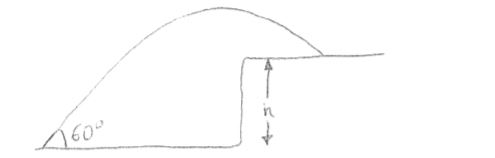
\includegraphics[scale=0.8]{ES1/FEB012016.jpg}
	\end{center}
\begin{boxed}
\null\hfill \textbf{Soluzione:} $y = 51.827 m$\\
\textbf{Procedimento: } \\
Scompongo la velocità $v_0$ sull'asse $y$\\
$v_{0,y}= v_0 \cdot \sin(\alpha) \quad = 42m/s\cdot \frac{\sqrt{3}}{2} \quad = 36.373m/s$ \\ \\
Calcolo con la formula del moto uniformemente accellerato la distanza percorsa sull'asse y \\
$y= y_0 + v_{0,y}\cdot t -\frac{1}{2}\cdot g \cdot t^2$\\
$y=0m+36.373m/s \cdot 5.5s -\frac{1}{2}\cdot 9.81 m/s^2 \cdot (5.5s)^2 = 200.051m - 148.225m = 51.827m$
\end{boxed}    
   
\end{figure}


\begin{figure}[h!]
\textbf{Tema d'Esame di Giugno 2016}\\ \\
Calcolare la velocità massima a cui un'auto che pesa 1000 kg riesce a percorrere una curva di raggio 85 m senza sbandare sapendo che il coefficiente d'attrito tra penumatico e asfalto è 0.7
\end{figure}


\begin{figure}[h!]
\textbf{Tema d'Esame di Luglio 2016}\\ \\
Una pallina viene lanciata come in figura con una velocità iniziale di 15 m/s e un
angolo $\theta$ di 60$^{\circ}$. Dopo quanto tempo atterrerà su un ripiano di altezza h = 4 m?
\\
	\begin{center}
		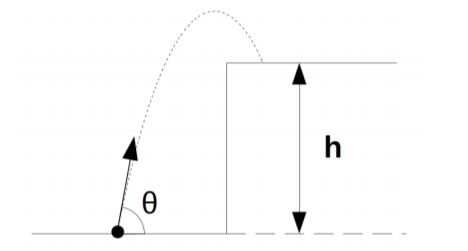
\includegraphics[scale=0.7]{ES1/LUG012016.jpg}
	\end{center}
\begin{boxed}
\null\hfill \textbf{Soluzione:} $x_2 = 2.29s m$\\
\textbf{Procedimento: } \\
Scompongo la velocità $v_0$ sull'asse $y$\\
$v_{0,y}= v_0 \cdot \sin(\alpha) \quad = 15m/s\cdot \frac{\sqrt{3}}{2} \quad = 12.99m/s$ \\ \\
Calcolo con la formula del moto uniformemente accellerato i tempi con il quale la pallina raggiunge l'altezza pari a $4m$ \\

$y= y_0 + v_{0,y}\cdot t -\frac{1}{2}\cdot g \cdot t^2$\\
$4m=0m+12.99m/s \cdot t -\frac{1}{2}\cdot 9.81 m/s^2 \cdot t^2 $\\
$4.905 t^2 -12.99t +4 $\\
$\Delta = 12.99^2-4 \cdot 4.905 \cdot 4 = 90.26 $\\
$ t_{1,2} = \frac{12.99 \pm \sqrt{90.26}}{2\cdot 4.905} = \quad t_1=0.356 \quad t_2=2.29$\\

Consideriamo $t_2$ perchè è il momento in cui tocca la terrazza, ossia a $2.29s$
\end{boxed}
\end{figure}
\clearpage


